\documentclass{article}

\usepackage{amsmath,amsfonts,amssymb}   

\newif\ifanswer
\answertrue
%\answerfalse

\let\imp=\Rightarrow
\let\iff=\Leftrightarrow
\usepackage{graphicx}
\usepackage{listings}
\usepackage{tikz-qtree}
\lstset{language=C}


\tikzset{every tree node/.style={minimum width=2em,draw,circle},
         blank/.style={draw=none},
         edge from parent/.style=
         {draw,->, edge from parent path={(\tikzparentnode) -- (\tikzchildnode)}},
         level distance=1.5cm}

\begin{document}

\section*{COMS10011 sample paper}

This is a sample paper, it has the same rubric and the same style of
question as the real paper, the layout is slightly different to the
official exam layout. 

\subsection*{Rubric}{
This paper contains \emph{two} parts. \\
The first section contains \emph {20} short questions.\\ 
Each question is worth \emph{two marks} and all should be attempted.\\
The second section contains \emph {three} long questions.\\
Each long question is worth \emph{25 marks}.\\
The best \emph{two} long question answers will be used for assessment. \\
The maximum for this paper is \emph{90 marks}. \\
Calculators must have the Faculty of Engineering Seal of Approval.}

%MSM: unit specific Latex commands 

\subsection*{Section A: short questions - answer all questions}

\begin{enumerate}

  %1
\item A coin is flipped four times. What is the sample space?

  \ifanswer
  Solution: 
  $\{TTTT,TTTH,TTHT,TTHH,THTT,THTH,THHT,$\\$THHH,HTTT,HTTH,HTHT,HTHH,HHTT,HHTH,HHHT,$\\$HHHH\}$.
  \fi


  %2
\item A probability is a map $P$ from events to real numbers. What are the three defining properties of a probability?

  \ifanswer
    Solution: 
\begin{enumerate}
\item $P(A)\ge 0$ for all events.
\item $P(X)=1$
\item If $A\cap B=\emptyset$ for two events $A$ and $B$ then 
\begin{equation}
P(A\cup B)=P(A)+P(B)
\end{equation}
\end{enumerate}
where $A\cap B$ and $A\cup B$ are the intersection and union of $A$
and $B$ and $\emptyset$ is the empty set.
\fi
  
%3
\item In stud poker you are given five cards from a normal pack of
  poker cards, that is with 13 cards labelled A, 2 to 10 and J, Q and
  K. Each value comes in one of four suits, spades, diamonds, clubs
  and hearts.  A straight has all the cards in order, for example
  A2345 or 56789. Even though A is the lowest card the sequence 10JQKA
  is allowed, however, A2345 and 10JQKA are the only two sequences
  allowed which include A. In a straight flush the cards are all the
  same suit. What is the probability of getting a straight flush? You may use
 $$
\left(\begin{array}{c}52\\5\end{array}\right)=\frac{52\times 51\times 50\times 49\times 48}{1\times 2 \times 3 \times 4\times 5}=2598960
  $$
  and the answer can be left as a fraction.

  \ifanswer
    Solution: 
    $$P=40/2598960=1/64974$$
    or if you exclude the royal flushes
    $$P=36/2598960$$
    either answer is acceptable.
  \fi

  %4
\item $X=\{1,2,3,4,5\}$ and $B=\{1,5\}$ what is $X\setminus B$?

  \ifanswer
    Solution: 
  $$x\setminus B = \{2,3,4\}$$
  \fi

  %5
\item In a library where all books have blue or yellow spines, four
  fifths of books with yellow spines are about mathematics but only
  a fifth of books with blue spines are about mathematics. There
  are the same number of yellow and blue spined books, you come upom a book open on a table; the book is about mathematics. What is the chance it has a yellow spine?

  \ifanswer
    Solution: In the obvious notation we need $p(M)$:
  $$p(M)=p(M|B)p(B)+p(M|Y)p(Y)=0.1+0.4=0.5$$
  and using Bayes:
  $$p(Y|M)=p(M|Y)p(Y)/p(M)=0.4/0.5=0.8$$
  \fi

  %6
\item Two four-sided dice are rolled and the two face values added up. Write down the probability table for the result.

  \ifanswer   Solution: $p(2)=1/16$, $p(3)=1/8$, $p(4)=3/16$, $p(5)=1/4$, $p(6)=3/16$, $p(7)=1/8$ and $p(8)=1/16$.
  \fi

  %7
  \item A six-sided dice is rolled five times, what is the chance of
    getting one exactly three times? You can leave your result as a fraction with powers.

    \ifanswer  Solution: 
    $$p=\left(\begin{array}{c}5\\3\end{array}\right)\frac{1}{6}^3\frac{5}{6}^2
      = \frac{20\times 5^2}{2\times 6^5}
      $$
      \fi

      %8
    \item On average three buses arrive at a bus stop every hour in the afternoon. What is the chance that no buses will arrive between 1pm and 2pm?

      \ifanswer  Solution: 
      $$p=e^{-3}$$
      \fi

      %9
    \item What is
      $$\lim_{n\rightarrow\infty}\left(1-\frac{x}{n}\right)^n$$

      \ifanswer
        Solution: 
      $$\lim_{n\rightarrow\infty}\left(1-\frac{x}{n}\right)^n=e^{-x}$$
        \fi
        
      %10
    \item If $F(x)$ is the cumulative for a continuous probability distribution, what is $\lim_{x\rightarrow\infty}F(x)$?

      \ifanswer
        Solution: 
      $$\lim_{x\rightarrow\infty}F(x)=1$$
  \fi
\item A Friedman test is a statistic test for comparing parametric data,
true or false? Explain yourself in one sentence.

\ifanswer
(Answer: False this is used for comparing non-parametric data, i.e. with a skewed distribution)
\fi

\item A researcher has created five new drugs (A B C D E) for weight loss and he wishes to verify which one is the best. He devises an experiment in which he tests the effect of each drugs on weight loss (number of grams lost). The researcher wants to use T-test in order to compare the effect of the drugs. Using Bonferroni corrections, what is the new significance level that the researcher should use when looking for significant results when comparing each pair?

\ifanswer
(Answer: 0.005/10 because there are 10 comparisons made)
\fi

\item A politician claims that the dropout rate for schools is less
  than 25\%. Last year, 190 out of 603 students dropped out. A
  researcher is aiming to looking for an evidence to reject the
  politician's claim, should he use a one tail or a two-tail
  statistical test and why?

\ifanswer
(Answer: one-tail is enough because the researcher is only interested in one direction. i.e. the dropout rate below 25\%. If the question was \lq{}equal to\rq{} we would use a two-tail test)
\fi

\item You are comparing two data sets and have done a two-tail
  unpaired t-test and the p-value returned is 0.08. How can you change
  the experimental design to increase your chances to have a p-values
  below the significant level of 0.05? Give two possible ways to do
  so.

\ifanswer  
(Answers possible: increase the sample size, used paired data (within subject experiment), design the experiment as one-tail)
\fi

\item One research is performing a crowd-source study to understand
  the effect of web advertising layouts on the number of items bought
  by a website visitor. He has gathered data from 5000 participants
  and he is trying to verify if the data are following a normal
  distribution. He is using a Shapiro-Wilk test to do this. Is this a
  correct method to test the assumption of normality? Yes or
  No. Explain why.

\ifanswer  
(Answer: False. Kolmogorov-Smirnov test is more appropriate for large sample size $N >50$ and Shapiro-Wilk for small sample size $N <=50$)
\fi

\item A scientist has found that the number of tornadoes since 2002
  follow a very similar pattern than the number of shark attacks since
  2002 (see graph). He claims that Tornadoes are causing the sharks to
  be stressed and to attack more people. Is the scientist's reasoning
  correct? Yes or no. Explain why.


  \ifanswer

  (Answer: No. The graphs show a correlation between the two data sets but not causality.  A correlation does not mean that the change in one variable is the cause of the change in the values of the other variable.
  \fi

\item Below is a list of variables that might be measured in a research study:
\begin{enumerate}
\item A person's length recorded in cm.
\item Whether a person is smoking, recorded as \lq{}Yes\rq{} or \lq{}No\rq{}.
\item How long a person worked for, recorded as the number of years.
\item The value of a house, recorded as \lq{}under \pounds 100 000\rq{}, \lq{}\pounds 100 000 - \pounds 500 000\rq{}, \lq{}\pounds 500 000 - \pounds 1 000 000\rq{}, \lq{}over \pounds 1 000 000\rq{}.
\item The treatment group a person was in, recorded as \lq{}Group 1\rq{}, \lq{}Group 2\rq{} and \lq{}Group 3\rq{}.
\item The change in concentration of sugar in a person's blood, recorded as a percentage of the original.
Write down whether each variable is categorical or numerical.
\end{enumerate}

\ifanswer
 (Answer: b, d, e are categorical; a, c, f are numerical.)
\fi

\item In a study, 20 participants were asked to write text using two
  different keyboard layouts: the classical QWERTY vs. a new one
  called DVORAK. DVORAK proponents claim the layout requires less
  finger motion and thus reduces errors compared to the standard
  QWERTY. Half of the participants started the task on the QWERTY
  layout and then the DVORAK and the other half of the participants
  started the task on the DVORAK layout and then the QWERTY. The
  number of words typed per minute was collected for each participant
  and each layout. Choose the most appropriate procedure to decide
  which layout allow participants to type the fastest.
  \begin{itemize}
    \item[A] Chi-squared test 
\item[B] Paired T-test
\item[C] Unpaired T-test
\item[D] Linear regression
  \end{itemize}
  
\ifanswer
(Answer: B)
\fi

\item In a study, 40 participants were randomized to two groups. One
  group received a drug to decrease hair loss and the other group
  received a placebo (a pill of sugar). At the end of the program, the
  percentage hair loss for each patient was recorded. Choose the most
  appropriate procedure to decide if there is a relationship between
  the use of the drug and the percentage of hair loss:
\begin{itemize}
\item[A] Chi-squared test 
\item[B] Paired T-test
\item[C] Unpaired T-test
\item[D] Linear regression
\end{itemize}

\ifanswer
(Answer: C)
\fi

\item A study attempted to find out if the age of an animal had any
  relationship to their athletic ability. The researchers took the
  data of 104 cheetahs, calculating their age and running a test to
  measure their speed. Choose the most appropriate procedure to decide
  if the age has any relationship with the run speed:
\begin{itemize}
\item[A] Chi-squared test
\item[B] Paired T-test
\item[C] Unpaired T-test
\item[D] Linear regression
\end{itemize}

\ifanswer
(Answer: D)
\fi

\end{enumerate}
  
\section*{Section B: long questions - answer two questions}

\begin{enumerate}

\item This question is largely about the binomial distribution.
  \begin{enumerate}
  \item{} [5] A six-sided dice is rolled four times. What is the change of getting exactly two threes?
      \item{} [5] A six-sided dice is rolled four times. What is the change of getting at least two threes?
    \item{} [5] An $n$-sided dice is rolled $s$ times with $n>3$. What is the change of getting exactly $r$ threes?
    \item{} [5] If the chance of getting exactly $r$ threes is $p(r)$ show
      $$\sum_{r=0}^sp(r)=1$$
    \item{} [5] You have a three-sided dice and a six-sided dice. In a game
      you flip a coin, if the coin comes up heads, you roll the
      three-sided dice, if it comes up tails, you roll the six-sided
      dice. What is the chance of getting a three.
      \end{enumerate}

\ifanswer
If a six sided dice if rolled four times then the probability of exactly two threes is
\begin{equation}
  p(2)=\left(\begin{array}{c}4\\2\end{array}\right)\left(\frac{1}{6}\right)^2\left(\frac{5}{6}\right)^2
\end{equation}
The chance of at least two threes is the same as the chance of anything except zero threes or one three:
\begin{equation}
  p(\ge 2)=1-\left(\frac{5}{6}\right)^4-4\left(\frac{1}{6}\right)\left(\frac{5}{6}\right)
\end{equation}
The more general case is
\begin{equation}
  p(r)=\left(\begin{array}{c}s\\r\end{array}\right)\left(\frac{1}{6}\right)^r\left(\frac{5}{6}\right)^{s-r}
\end{equation}
The sum of $p(r)$ is one follows from the binomial theorem
\begin{equation}
  (p+q)^s=\sum_{r=0}^s\left(\begin{array}{c}s\\r\end{array}\right)p^rq^{s-r}
\end{equation}
but with $q=1-p$. Finally the probability of getting a three in the coin flipping game is
\begin{equation}
  p=\frac{1}{2}\frac{1}{6}+\frac{1}{2}\frac{1}{3}
\end{equation}
\fi

\item This question has two parts, one is about Bayes's theorem, the other about Pearson's chi-square test.

  \begin{enumerate}
  \item{} [10] You want to go for a walk. However, when you wake up the day is cloudy and half of all raining days start of cloudy. On the other hand, two days in five start off cloudy and it's been rather dry recently with only rain only on one day in ten. What is the chance it will rain?
\item{} [15]  A genetics engineer was attempting to cross a tiger and a cheetah. She predicted a phenotypic outcome of the traits she was observing to be in the following ratio: 4 stripes only; 3 spots only; 9 both stripes and spots. When the cross was performed, and she counted the individuals she found 50 with stripes only, 41 with spots only and 85 with both. According to the Chi-square test, did she get the predicted outcome? Use the table below with a significance level of 0.05 to check. 

	\begin{center}
		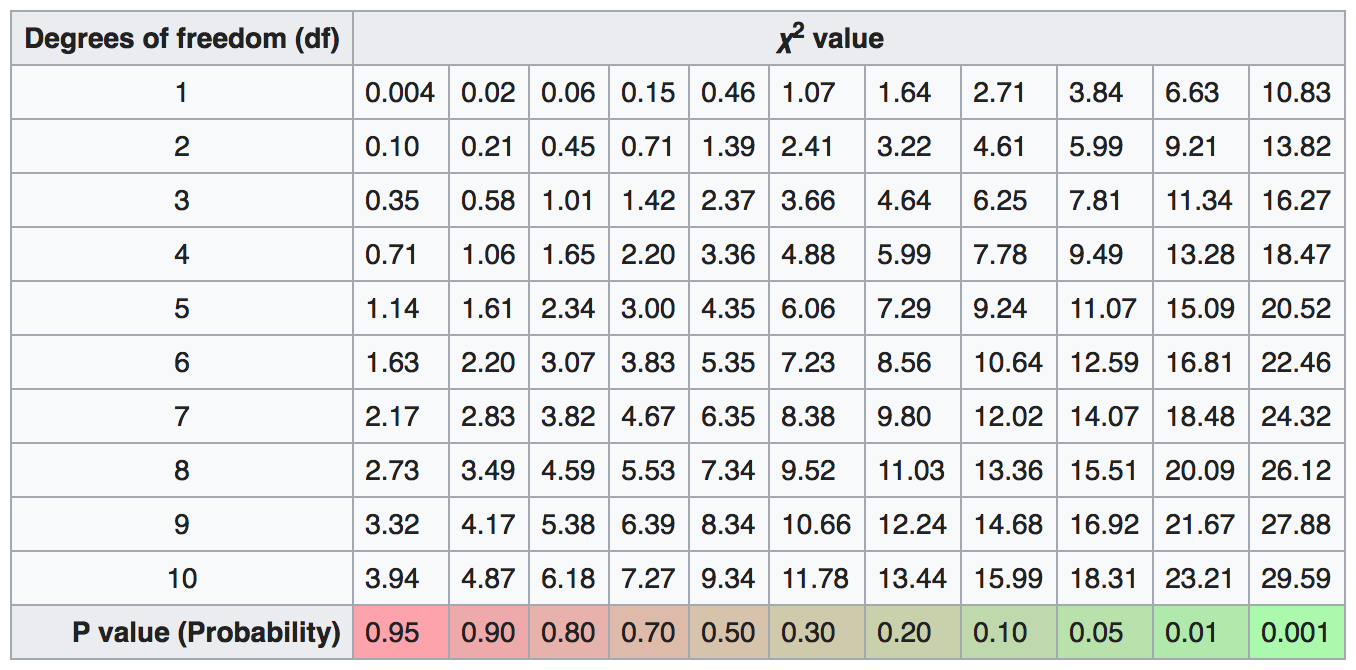
\includegraphics[width=5.5in]{chi-square.png}
	\end{center}
\end{enumerate}
  
    \ifanswer
    For the Bayes question
    \begin{equation}
      p(\mbox{rain}|\mbox{cloudy})=\frac{p(\mbox{cloudy}|\mbox{rain})p(\mbox{rain})}{p(\mbox{cloudy})}=\frac{0.5*0.1}{0.4}=0.125
    \end{equation}
    For the chi-square question
    \begin{center}
      \begin{tabular}{|l|c|c|c|c|c|}
        \hline
        \mbox{expected ratio}&\mbox{observed \#}&\mbox{expected \#}&$O-E$&$(O-E)^2$&$(O-E)^2/E$\\
        \hline
        \mbox{4 stripe}&50&44&6&36&0.82\\
        \mbox{3 spots}&41&33&8&64&1.94\\
        \mbox{9 stripes/spots}&85&99&-14&196&1.98\\
        \hline
        \mbox{total}&176&176&0&&4.74\\
        \hline
      \end{tabular}
    \end{center}
    where $4/16*176=44$, $3/16*176=33$, $9/16*176=99$ and the degrees
    of freedom are $3-1=2$ since there are three characteristics:
    spots, stripes and both. $4.74$ is less than $5.991$ so we can accept the null hypothesis.

    \fi

\item You have designed a horror game in which a sound of heartbeat is
  played during the game. Your assumption is that the sound of the
  heartbeat make the game frightening. You wish to design an
  experiment to investigate if adding the sound of the heartbeat does
  increase the actual heartbeat of the player. You set out to make 20
  participants play two versions of your game: one with the sound of
  heartbeat is played, one with no sound. Using a heartbeat sensor,
  you measure the heart rate of the participants before playing and
  after and note the difference.
\begin{enumerate}
\item{} [6] What are your independent and dependent variables

\ifanswer  
Answer: dependant = different in heartbeat / independent = sound of heartbeat or not
\fi

\item{} [8] Are you doing a within or between experiment and why?

\ifanswer
Answer: it is possible to do a within-subjects experiment as long as the portion of the game tested are changed between the sound vs. no sound. You would have to make sure the portion of the game used are comparable (same level of fear). Doing it within would be better because the data are paired and thus you would need less participants. You can also do a between-subjects study in which one group of participants would test the same portion of the game with sound and another group of participants would test it without. In such case you will be surer that the games are comparable (in term of level of fear) but you will need more participants.
\fi

\item{} [6] Do you need to use counterbalancing or not and why?

\ifanswer
Answer: in the within case, you would need to make one half of the participants start with the \lq{}no sound\rq{} condition and then the \lq{}sound\rq{} one. The other half of participants would do the opposite.
\fi

\item{} [5] Imagine what is the task that the participants are going to do. [4 marks]

\ifanswer Answer: the participants are asked to sit down in front of
the TV screen and to take the Xbox controller. The experimenter first
measures the participants rest heartbeat. The game starts, and the
participants are asked to find a specific item in the game. Once
finished the experimenter measures the participants current heartbeat.
\fi
\end{enumerate}

 \end{enumerate}
  
\end{document}
